\section{Auswertung}
\label{sec:Auswertung}

\subsection{Bestimmung der mittleren Reichweite und Energie zweier Messreihen}

Die Abstände $x_0$ zwischen $\alpha$-Strahler und Detektor betragen für die Messreihen
$\SI{2.4}{\centi\meter}$ und $\SI{2.9}{\centi\meter}$. Für diese Abstände werden jeweils
$100$ Messungen der Zählrate $N$ und des Energiemesschannels für den Druck zwischen
$\SI{0}{\milli\bar}$ und $\SI{1000}{\milli\bar}$ und einer Zeitspanne von
$t = \SI{120}{\second}$ durchgeführt. 

Daraus kann der effektive Abstand $x_\text{eff}$ nach der Formel \eqref{eqn:Weglaenge}
berechnet werden. Die Energie wird dadurch bestimmt, dass der jeweils höchste Channel dem
Energiewert $\SI{4}{\mega\eV}$ entspricht und die restlichen Channel und Energien
proportional dazu sind.

Der erste Messwert der Zählrate wird $N_0$ benannt.

\subsubsection{Messreihe 1} %1111111111111111111111111111111111111111111111111111111

Für die erste Messreihe beträgt $x_0 = \SI{2.4}{\centi\meter}$. Die zugehörigen
Messwerte und berechneten effektiven Abstände $x_\text{eff}$ und Energien $E$ sind in
Tabelle \ref{tab:mess1} aufgelistet.

\begin{table}
  \centering
  \caption{Werte der gemessenen Zählrate, Energien und des effektiven Abstandes für 
            $x_0 = \SI{2.4}{\centi\meter}$ (Messreihe 1)}
  \label{tab:mess1}
  \sisetup{table-format=2.1}
  \begin{tabular}{c c c c c}
  \toprule
  $p \,/\, \si{\milli\bar}$ & $N$ & Channel & $x_\text{eff} \,/\, \si {\centi\meter}$ & 
  $E \,/\, \si{\mega\eV}$\\
  \midrule 
         0 & 74494 & 783 & 0,00 & 4,00 \\
        50 & 74222 & 775 & 0,12 & 3,96 \\
       100 & 73453 & 711 & 0,24 & 3,63 \\
       150 & 73055 & 706 & 0,36 & 3,61 \\
       200 & 72618 & 655 & 0,47 & 3,35 \\
       250 & 72194 & 675 & 0,59 & 3,45 \\
       300 & 72125 & 688 & 0,71 & 3,51 \\
       350 & 71052 & 655 & 0,83 & 3,35 \\
       400 & 70683 & 632 & 0,95 & 3,23 \\
       450 & 69756 & 655 & 1,07 & 3,35 \\
       500 & 68126 & 591 & 1,18 & 3,02 \\
       550 & 67015 & 583 & 1,30 & 3,00 \\
       600 & 65616 & 527 & 1,42 & 2,69 \\
       650 & 61699 & 511 & 1,54 & 2,61 \\
       700 & 57008 & 399 & 1,66 & 2,04 \\
       750 & 46274 & 399 & 1,78 & 2,04 \\
       800 & 35333 & 399 & 1,90 & 2,04 \\
       850 & 21152 & 399 & 2,10 & 2,04 \\
       900 &  8363 & 399 & 2,13 & 2,04 \\
       950 &  3849 & 397 & 2,25 & 2,03 \\
      1000 &  1738 & 395 & 2,37 & 2,02 \\
  \bottomrule
  \end{tabular}
  \end{table}

Zur Bestimmung der mittleren Reichweite sind in Abbildung \ref{fig:plot1} die Messwerte der Zählrate $N$ 
gegen den effektiven Abstand $x_\text{eff}$ abbgebildet.

\begin{figure} [H]
  \centering
  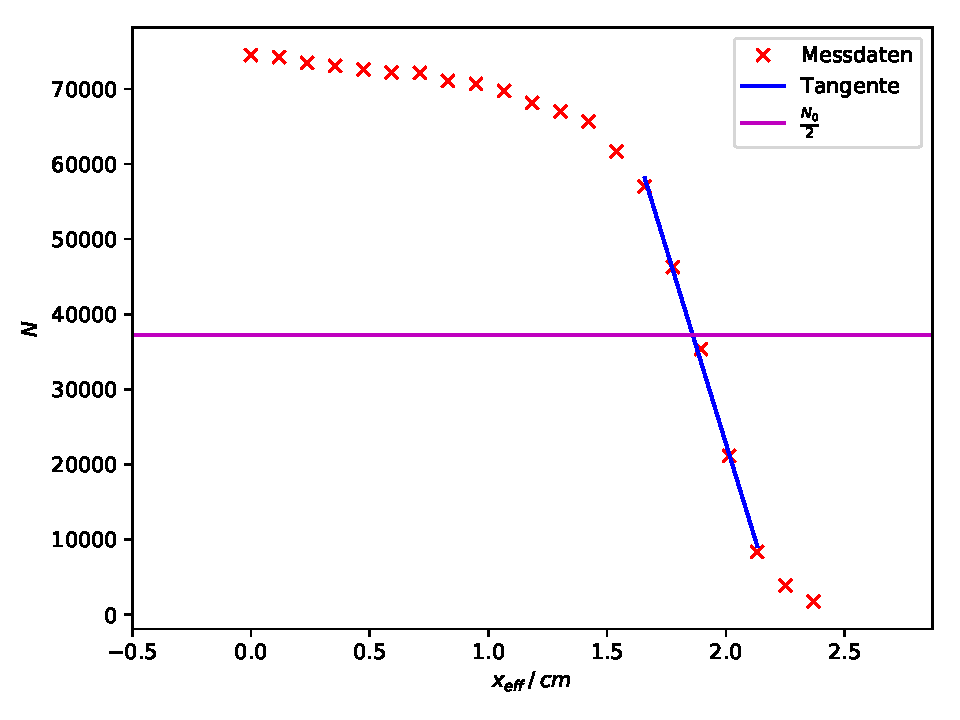
\includegraphics[scale=0.8]{content/plot1.pdf}
  \caption{Bestimmung der mittleren Reichweite aus der Messung der Zählrate (Messreihe 1)}
  \label{fig:plot1}
\end{figure}

Für das Intervall von $x_\text{eff} = \SI{1.66}{\centi\meter}$ bis $x_\text{eff} = \SI{2.13}{\centi\meter}$
wird mittels python eine Lineare Regression der Form $N(x_\text{eff}) = a x_\text{eff} + b$ durchgeführt,
die die Parameter 

\begin{align*}
    a &= \SI{- 103336.13 +- 5941.49}{\per \centi \meter} \\
    b &= 229485,20 \pm 11305,16
\end{align*}

enthält. Durch die Schnittstelle der Regressionstangente und der Konstante $\frac{N_0}{2} = 37247$,
kann die mittlere Reichweite als

\begin{equation*}
    R_{m,1} = \frac{\frac{N_0}{2} - b}{a} = \SI{1.86 +- 0.15}{\centi\meter}
\end{equation*}

bestimmt werden.

Nach Umstellung der Formel \eqref{eqn:energie} ergibt sich die Energie 

\begin{equation*}
     E_{\alpha, 1} = \SI{3.30 +- 0.18}{\mega\eV} \; .
\end{equation*}

Weiterhin werden die Energiemesswerte in Abbildung \ref{fig:plot2} gegen $x_\text{eff}$ aufgetragen.

\begin{figure} [H]
  \centering
  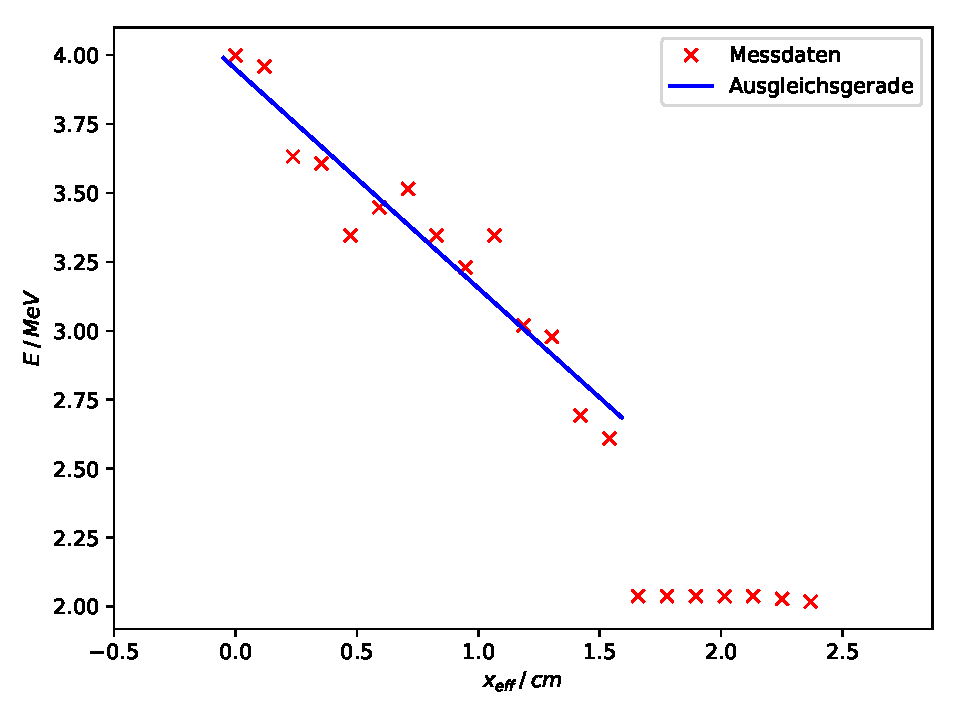
\includegraphics[scale=0.8]{content/plot3.pdf}
  \caption{Bestimmung der Energieänderung aus den Energiemesswerten (Messreihe 1)}
  \label{fig:plot2}
\end{figure}

Die Lineare Regression mittels python der Form $E(x_\text{eff}) = c x_\text{eff} + d$ im Intervall
von $x_\text{eff} = \SI{0.00}{\centi\meter}$ bis $x_\text{eff} = \SI{1.54}{\centi\meter}$
ergibt die Parameter

\begin{align*}
  c &= \SI{- 0.795 +- 0.079}{\mega \eV \per \centi \meter} \\
  d &= \SI{3.949 +- 0.072}{\mega\eV} \; .
\end{align*}

Danach ergeben sich die Energieänderung und mittlere Energie zu

\begin{align*}
  \frac{dE_{\alpha, 1}}{dx} &= c = \SI{-0.795 +- 0.079}{\mega \eV \per \centi \meter} \\
  E_{\alpha, R_{\alpha, 1}} &= E(R_{\alpha, 1}) = \SI{2.47 +- 0.20}{\mega\eV} \; .
\end{align*}


\subsubsection{Messreihe 2} %2222222222222222222222222222222222222222222222222222222222222222222222

Für die zweite Messreihe beträgt $x_0 = \SI{2.9}{\centi\meter}$. Die zugehörigen
Messwerte und berechneten effektiven Abstände $x_\text{eff}$ und Energien $E$ sind in
Tabelle \ref{tab:mess2} aufgelistet.


  \begin{table}
    \centering
    \caption{Werte der gemessenen Zählrate, Energien und des effektiven Abstandes für 
              $x_0 = \SI{2.9}{\centi\meter}$ (Messreihe 2)}
    \label{tab:mess2}
    \sisetup{table-format=2.1}
    \begin{tabular}{c c c c c}
    \toprule
    $p \,/\, \si{\milli\bar}$ & $N$ & Channel & $x_\text{eff} \,/\, \si{\centi\meter}$ & 
    $E \,/\, \si{\mega\eV}$\\
    \midrule 
         0 & 58503 & 786 & 0,00 & 4,00 \\
        50 & 57901 & 743 & 0,14 & 3,78 \\
       100 & 57694 & 751 & 0,29 & 3,82 \\
       150 & 57484 & 727 & 0,43 & 3,70 \\
       200 & 56789 & 726 & 0,57 & 3,69 \\
       250 & 56298 & 655 & 0,72 & 3,33 \\
       300 & 55741 & 655 & 0,86 & 3,33 \\
       350 & 55224 & 635 & 1,00 & 3,23 \\
       400 & 54193 & 611 & 1,15 & 3,11 \\
       450 & 53258 & 547 & 1,29 & 2,78 \\
       500 & 51560 & 583 & 1,43 & 2,97 \\
       550 & 49368 & 519 & 1,57 & 2,64 \\
       600 & 44862 & 480 & 1,72 & 2,44 \\
       650 & 37475 & 399 & 1,86 & 2,03 \\
       700 & 25972 & 399 & 2,00 & 2,03 \\
       750 & 14061 & 399 & 2,15 & 2,03 \\
       800 &  4752 & 393 & 2,29 & 2,00 \\
       850 &  1576 & 392 & 2,43 & 2,00 \\
       900 &   921 & 393 & 2,58 & 2,00 \\
       950 &   686 & 391 & 2,72 & 1,99 \\
      1000 &   712 & 391 & 2,86 & 1,99 \\
    \bottomrule
    \end{tabular}
    \end{table}

    Zur Bestimmung der mittleren Reichweite sind in Abbildung \ref{fig:plot3} die Messwerte der Zählrate $N$ 
    gegen den effektiven Abstand $x_\text{eff}$ abbgebildet.
    
    \begin{figure} [H]
      \centering
      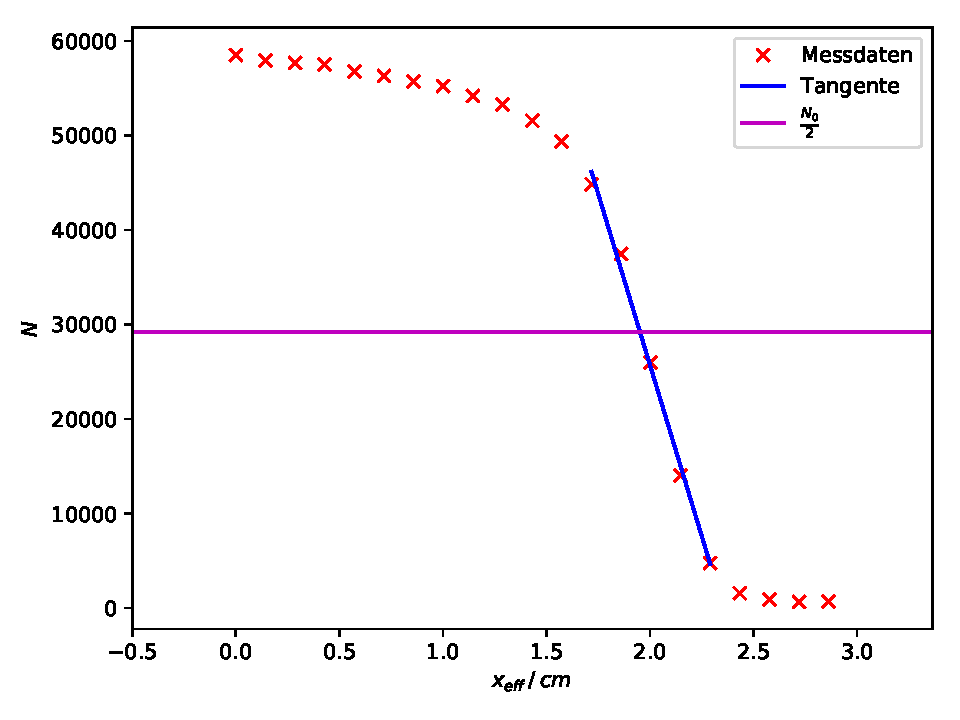
\includegraphics[scale=0.8]{content/plot2.pdf}
      \caption{Bestimmung der mittleren Reichweite aus der Messung der Zählrate (Messreihe 2)}
      \label{fig:plot3}
    \end{figure}
    
    Für das Intervall von $x_\text{eff} = \SI{1.72}{\centi\meter}$ bis $x_\text{eff} = \SI{2.29}{\centi\meter}$
    wird mittels python eine Lineare Regression der Form $N(x_\text{eff}) = a x_\text{eff} + b$ durchgeführt,
    die die Parameter 
    
    \begin{align*}
        a &= \SI{- 72400.86 +- 5325.81}{\per \centi \meter} \\
        b &= 170512,00 \pm 10726,97
    \end{align*}
    
    enthält. Durch die Schnittstelle der Regressionstangente und der Konstante $\frac{N_0}{2} = 29251,5$,
    kann die mittlere Reichweite als
    
    \begin{equation*}
        R_{m,2} = \frac{\frac{N_0}{2} - b}{a} = \SI{1.95 +- 0.21}{\centi\meter}
    \end{equation*}
    
    bestimmt werden.
    
    Nach Umstellung der Formel \eqref{eqn:energie} ergibt sich die Energie 
    
    \begin{equation*}
         E_{\alpha,2} = \SI{3.41 +- 0.24}{\mega\eV} \; .
    \end{equation*}
    
    Weiterhin werden die Energiemesswerte in Abbildung \ref{fig:plot4} gegen $x_\text{eff}$ aufgetragen.
    
    \begin{figure} [H]
      \centering
      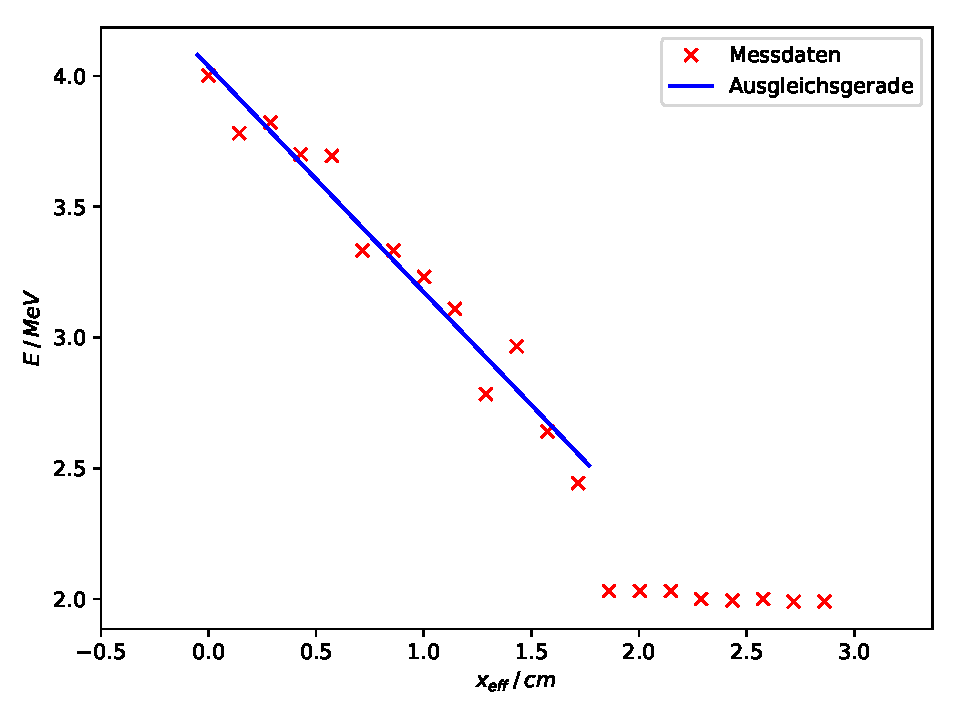
\includegraphics[scale=0.8]{content/plot4.pdf}
      \caption{Bestimmung der Energieänderung aus den Energiemesswerten (Messreihe 2)}
      \label{fig:plot4}
    \end{figure}
    
    Die Lineare Regression mittels python der Form $E(x_\text{eff}) = c x_\text{eff} + d$ im Intervall
    von $x_\text{eff} = \SI{0.00}{\centi\meter}$ bis $x_\text{eff} = \SI{1.72}{\centi\meter}$
    ergibt die Parameter
    
    \begin{align*}
      c &= \SI{- 0.863 +- 0.060}{\mega \eV \per \centi \meter} \\
      d &= \SI{3.949 +- 0.061}{\mega\eV} \; .
    \end{align*}
    
    Danach ergeben sich die Energieänderung und mittlere Energie zu
    
    \begin{align*}
      \frac{dE_{\alpha, 2}}{dx} &= c = \SI{-0.863 +- 0.060}{\mega \eV \per \centi \meter} \\
      E_{\alpha, R_{\alpha, 2}} &= E(R_{\alpha, 2}) = \SI{2.27 +- 0.22}{\mega\eV} \; .
    \end{align*}


   \subsection{Statistik des radioaktiven Zerfalls} %3333333333333333333333333333333333333333333333333333333333333

      Zur statistischen Untersuchung sind für den Druck $p = \SI{0}{\milli\bar}$ $n = 100$ Messwerte der
      Zählrate $N$ in Tabelle \ref{tab:mess3} aufgelistet.

    \begin{table}
      \centering
      \caption{100 statistische Messwerte der Zählrate bei $p = \SI{0}{\milli\bar}$ und Abstand 
          $x = \SI{2.9}{\centi\meter}$}
      \label{tab:mess3}
      \sisetup{table-format=2.1}
      \begin{tabular}{c c c c c}
      \toprule
          4643 & 4535 & 4447 & 4700 & 4674 \\
          4748 & 4488 & 4487 & 4721 & 4504 \\
          4635 & 4431 & 4669 & 4246 & 4706 \\
          4559 & 4698 & 4512 & 4603 & 4414 \\
          4386 & 4781 & 4946 & 4813 & 4547 \\
          4537 & 4867 & 4808 & 4895 & 4450 \\
          4627 & 4460 & 4854 & 4575 & 4568 \\
          4737 & 4717 & 4847 & 4459 & 4692 \\
          4645 & 4662 & 4411 & 4964 & 4801 \\
          4405 & 4624 & 4522 & 4462 & 4654 \\
          4642 & 4579 & 4544 & 4624 & 4699 \\
          4374 & 4516 & 4826 & 4646 & 4729 \\
          4542 & 4879 & 4455 & 4584 & 4410 \\
          4834 & 4419 & 4780 & 4522 & 4559 \\
          4600 & 4827 & 4687 & 4373 & 4629 \\
          4874 & 4420 & 4576 & 4566 & 4507 \\
          4554 & 4669 & 4503 & 4680 & 4758 \\
          4554 & 4348 & 4231 & 4751 & 4345 \\
          4607 & 4615 & 4655 & 4573 & 4762 \\
          4590 & 4385 & 4630 & 4385 & 4606 \\
      \bottomrule
      \end{tabular}
      \end{table}

    Zunächst werden der Mittelwert $\mu$ und die Standartabweichung $\sigma$ berechnet:

    \begin{align}
        \mu &= \frac{1}{n} \sum_{i=1}^n N_i = 4605,59 \\
        \sigma &= \sqrt{ \frac{1}{n-1} \sum_{i=1}^n (N_i - \mu)^2  } \; .
    \end{align}

    Die Messwerte sind in Abbildung \ref{fig:plot5} gaußverteilt in einem Histogramm dargestellt.
    Zusätzlich abbgebildet ist die zugehörige Gaußverteilung der Form

    \begin{equation}
        G(N, \mu, \sigma) = \frac{1}{\sigma \sqrt{2 \pi}} \cdot \text{exp} 
                            \left(- \frac{(N - \mu)^2}{2 \sigma^2} \right) \; .
    \end{equation}

    \begin{figure} [H]
      \centering
      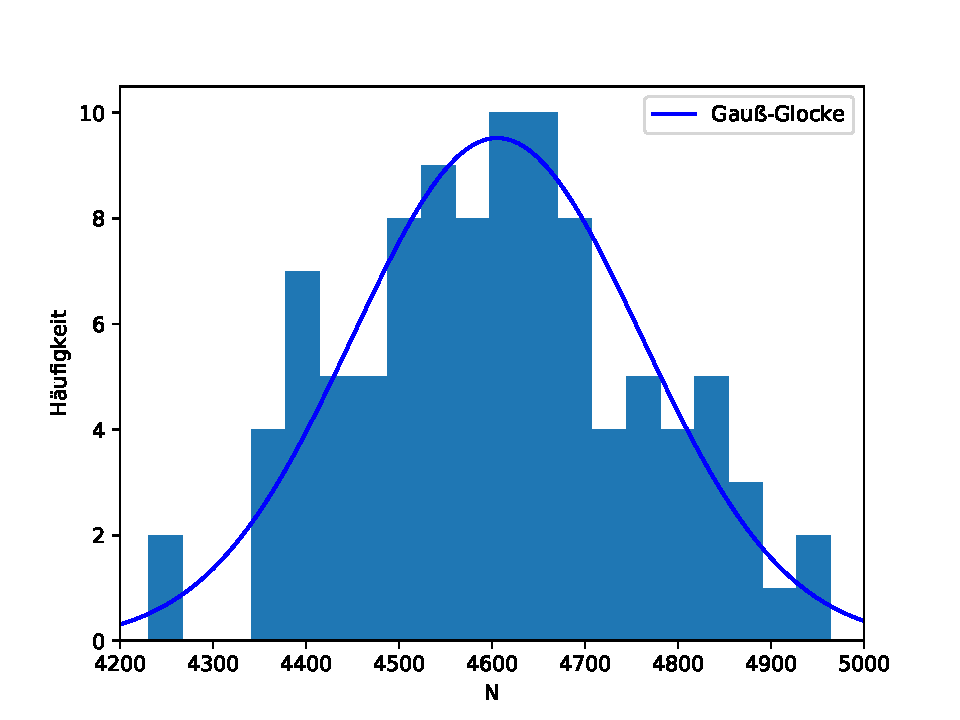
\includegraphics[scale=0.8]{content/gauss.pdf}
      \caption{Gaußverteilte Messwerte der Zählrate}
      \label{fig:plot5}
    \end{figure}


    Zusätzlich werden die Messwerte für eine Poissonverteilung normiert:

    \begin{equation}
        N_\text{i, norm} = \frac{N_i - N_\text{min}}{n} \; .
    \end{equation}

    Dabei beschreibt $N_{min} = 4231$ den kleinsten der gemessenen Zählratenwerte $N_i$.
    Durch die Normierung liegen die Werte $M$ nun zwischen $0$ und $7$.
    Ihr Mittelwert beträgt $\mu_P = 3,72$.
    Die poissonverteilten Werte sind nun zusammen mit der theoretischen Poissonverteilung

    \begin{equation}
        p_{\mu_P}(M) = \frac{\mu_P^M}{M!} \cdot \text{e}^{-\mu_P} 
    \end{equation}

    in Abbildung \ref{fig:plot6} abbgebildet.

    \begin{figure} [H]
      \centering
      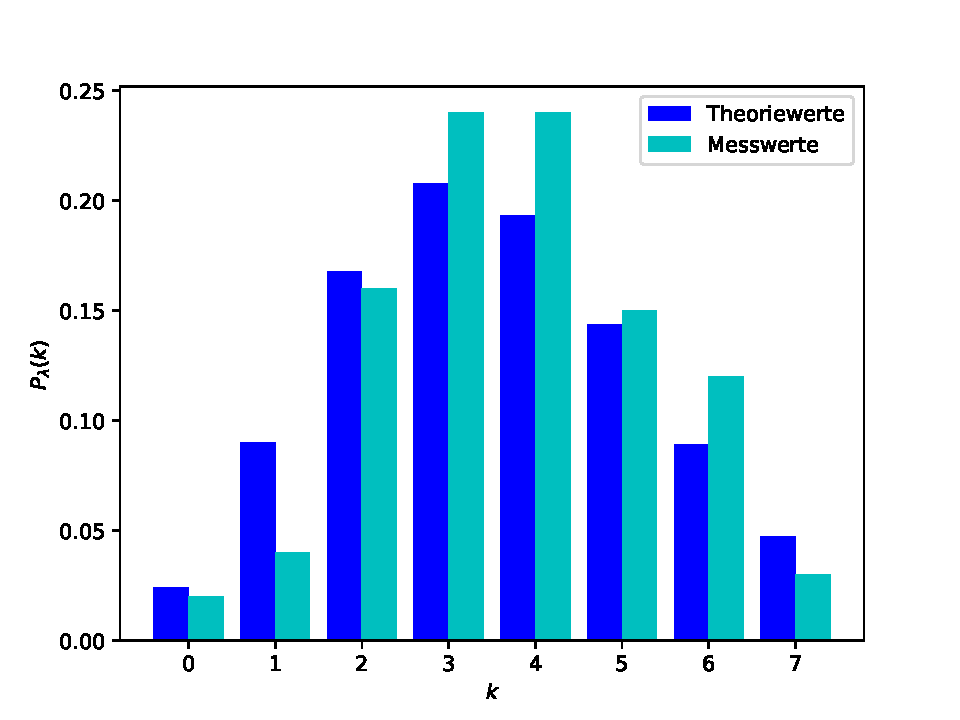
\includegraphics[scale=0.8]{content/poisson.pdf}
      \caption{Poissonverteilte Messwerte der Zählrate}
      \label{fig:plot6}
    \end{figure}
